\chapter{Systems Engineering}

\section{System}
A purposeful collection of inter-related components working together to achieve some common objective.\\[0.5ex]
\textbf{System categories:} (1) Technical computer-based systems (2)Socio-technical systems.

Systems engineering is the activity of specifying, designing, implementing, validating, deploying and maintaining socio-technical systems. Systems engineers are not just concerned with software but also with hardware and the system's interactions with users and its environment.

\subsection{Legacy Systems}
Legacy systems is an old or out-dated system, technology or software
application that continues to be used by an organization because it still performs the functions it was initially intended to do. For example: Windows 7, COBOL, Oracle database.

\begin{figure}[H]
   \centering
   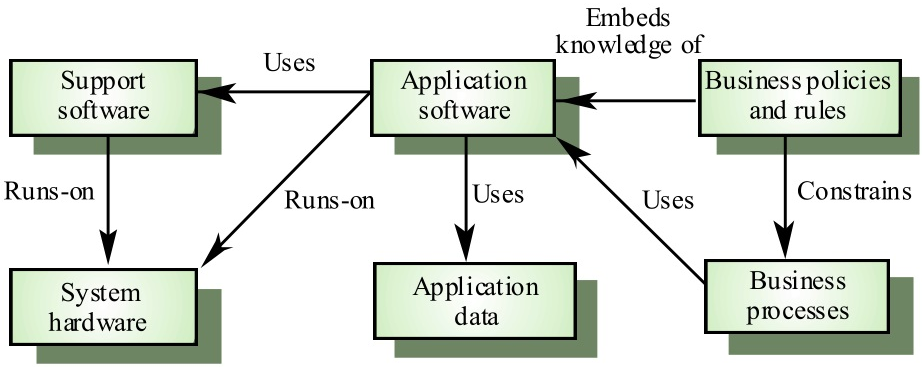
\includegraphics[width=0.6\textwidth]{figures/legacy-system.png}
   \caption{\small{Computer System Components}}
\end{figure}

\subsubsection*{Layered Model:}
Business process $\to$ Application Software $\to$ Support Software $\to$ Hardware.

\subsubsection*{Challenges changing a legacy system:}
(1) Costs
(2) Technical specifications
(3) Data protection
(4) User experience.

\subsubsection*{Top Legacy System Modernization Trends}

Automation, DevOps, Container-Based Applications, Microservice Architecture

\subsection{Critical System}

It is the systems that fail to deliver the expected objective in which any system failure can result in economic losses, physical damage or human life loss.

\textbf{There are three main types of critical systems:}
\begin{itemize}[parsep=1ex]
   \item \textbf{Safety-critical systems:}\\
   Failure results in loss of life, damage to the environment;
   e.g: Chemical plant protection system.

   \item \textbf{Mission-critical systems:}\\
   Failure results in failure of some goal-directed activity;
   e.g: Spacecraft navigation system.

   \item \textbf{Business-critical systems:}\\
   Failure results in high economic losses;
   e.g: Bank accounting system.
\end{itemize}


\subsection{System Dependability}
The dependability of a system reflects the user's degree of trust in
that system. It reflects the extent of the user's confidence that it
will operate as users expect and that it will not 'fail' in normal use.

\textbf{Principal dimensions of dependability are:}\\[1ex]
Availability, 
Reliability, 
Safety, 
Security, 
Repairability, 
Maintainability, 
Survivability, 
Error tolerance


\section{Software Development Life Cycle}

SDLC stands for Software Development Lifecycle. SDLC is a systematic process for building software that ensures the quality and correctness of the software built. SDLC process aims to produce high-quality software that meets customer expectations.

\subsection*{SDLC Phases}

\begin{enumerate}[label=Phase \arabic*:,left=0pt,itemsep=0.5ex]
   \item \textbf{Requirement Analysis:} Requirements Gathering to get detailed and precise requirements.
   
   \item \textbf{Feasibility study:}
   Operational, Technical, Economic, Schedule, Legal.
   \item \textbf{Design:}
   System and software design documents are created as
   per the SRS document. High/Low level design.
   \item \textbf{Coding:} developers start build the entire system by writing code.
   
   \item \textbf{Testing:} Tested until the software is bug-free, stable, and working as per the business needs.
   
   \item \textbf{Deployment:} The final software is released and checked for deployment issues.
   
   \item \textbf{Maintenance:} Bug fixing, Upgrade, Enhancement.
\end{enumerate}